\DiaryEntry{Maximum Likelihood Estimation of Bernoulli Variables}{2017-02-20}{Stochastic}

We have a coin showing H(head) with probability $p$ or T(ail) (with probability $1-p$) and observe a sequence of $N$ coin throws (e.g. ``HHTHHTT''). The sequence contains $H$ heads and $T = N-H$ tails.

The probability $P(H,T;p)$ for such a sequence is

\bee
P(H,T;p) = {N \choose{T}} p^T (1-p)^H
\eee

Based on this observation we want to perform maximum-likelihood estimation of the distribution parameter $p$. We take the first derivative

\bee
\frac{dP(H,T;p}{dp} = c H p^{H-1} (1-p)^T + c p^H T (1-p)^{T-1}(-1)
\eee

where $c = {N \choose{T}}$. We set the derivative to zero and solve for $p$,

\bee
H p^{H-1} (1-p)^T - p^H T (1-p)^{T-1} = 0 \rightarrow H (1-p) = Tp
\eee

and obtain

\bee
p^\star = \frac{H}{H+T} = \frac{H}{N}
\eee

Intuitively, this seems to make sense: The esimtated probability is the number of heads divided by the number of coin throws.


\subsubsection{Example}

The Figure \ref{2017-02-20:fig1} shows the value of $P(H,T;p)$ as function of $p$ for different dice sequences. It can be seen that the maximum of the probability for sequences with more heads than tails is shifted to the right. In case of an equal number of heads and tails, the maximum is located at $p=0.5$. A larger number of observations causes a ``peakier'' distribution.

\begin{figure}[htb!]
\label{2017-02-20:fig1}
\centering
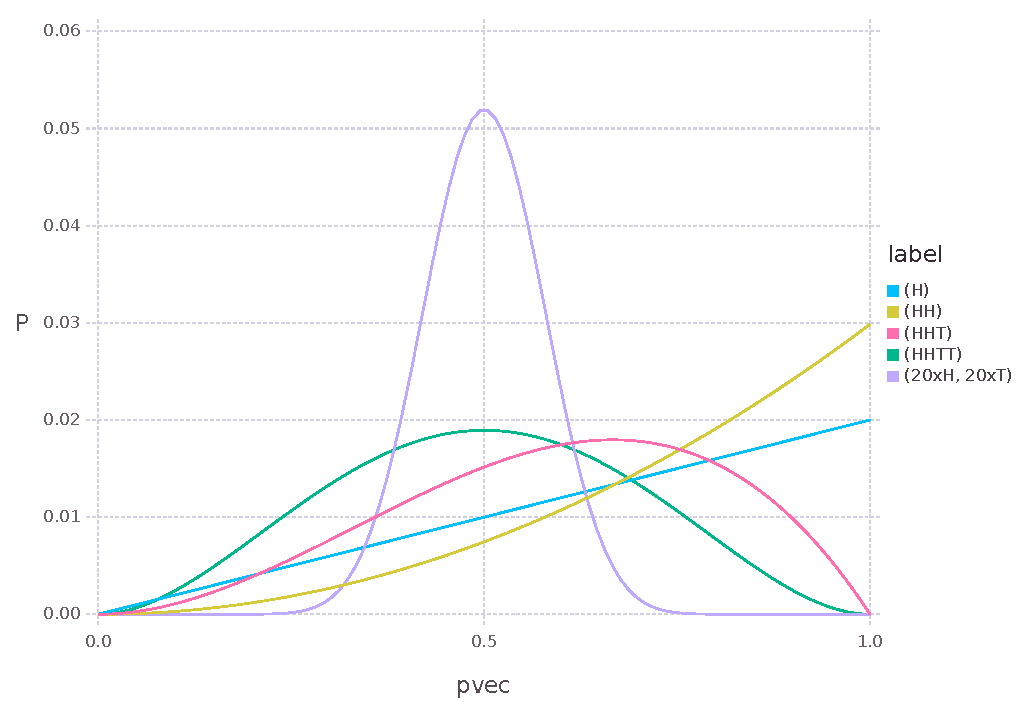
\includegraphics[scale=0.8]{images/bernoulli_est.eps}
\caption{Value of $P(H,T;p)$ as function of $p$ for different dice sequences.}
\end{figure}

